\begin{proof}
    In this exercise, I have to describe the various steps of the genetic algorithm that can be used. Subsequently, I can simulate it to check whether it's working or not.\par
    First, I will use the encoding scheme used in \cite{axelrod}: I describe it in somewhat detail here. For each move in the game, there are four possibilities: both players can cooperate (C or R for reward), the second player can defect while the first cooperates (CD or S for sucker), the first player can defect while the second cooperates (DC or T for temptation), or both players can defect (DD or P for penalty). To code a particular strategy, the particular behavioral sequence is coded as a three-letter string. For example, RRR would represent the sequence where both players cooperated over the previous three moves and SSP would represent the sequence where the first player was played for a sucker twice, and then finally defected. This three-letter sequence is then used to generate a number between 0 and 63, by interpreting it as a number in base 4. One such possible way is to assign
    a digit value to each of the characters in following way: DD = P = 0, DC = T = 1, CD = S = 2, and CC = R = 3. In this way, PPP would decode to 0, and SSR will decode to \(2\cdot4^2 + 2 \cdot 4^1 + 3 \cdot 4^0 = 43\). With the knowledge of these past three moves, a player will then require one of two possible moves (a cooperate “C” or a defect “D”) to be supplied by a GA solution. With these two options in each of 64 positions, a particular strategy can be defined by a 64-bit binary GA string of C (cooperate) and D (defect), where the ith C or D corresponds to the ith behavioral sequence dictated by the three-letter sequence of past three moves. Since a particular move depends on the previous three moves, the first three moves in a game are undefined in the above scheme. To account for these moves, six bits (with C and D, initially assigned at random) are appended to the above 64-bit string to specify a strategy’s premises, or assumption about the pre-game behavior. Together, each of the 70-bit strings thus represent a particular strategy, the first 64 are used for rules and the next six are used for the premises.\par
    For the initialization process, I can simply initialize the population with some random 70-bits strings.\par
    In order to evaluate a chromosome (that is, a strategy), I decided to play 100 games against a player that uses the well known \emph{tit-for-tat} strategy (an agent using this strategy will first cooperate, then subsequently replicate an opponent's previous action). Specifically, if \(s(j), j=1,2,\dots,100\) is the score of the j-th game that a player attains using the strategy defined by the chromosome, then the fitness value related to the chromosome is given by \(100\cdot 6 - \sum_{j=1}^{100}s(j)\). We would like to find the strategy that maximizes that value.\par
    For the selection process, I decided to use the simple \emph{roulette wheel with slots}.\par
    The crossover and the mutation operators are defined as usual, since I'm working with arrays of bits, and since every possible array is a valid one.\par
    There are no stopping conditions for the algorithm. Instead, it's possible to perform a fixed number of iterations.\par
    I have implemented this genetic algorithm and I performed an experiment with it. I've used \(p_c = 0.5\) (crossover probability), \(p_m = 0.001\) (mutation probability) and \(n = 50\) (number of individuals). I've generated 1000 generations, tracking the best strategy among all the generations and the average fitness value associated to each generation.\par
    \begin{figure}
        \centering
        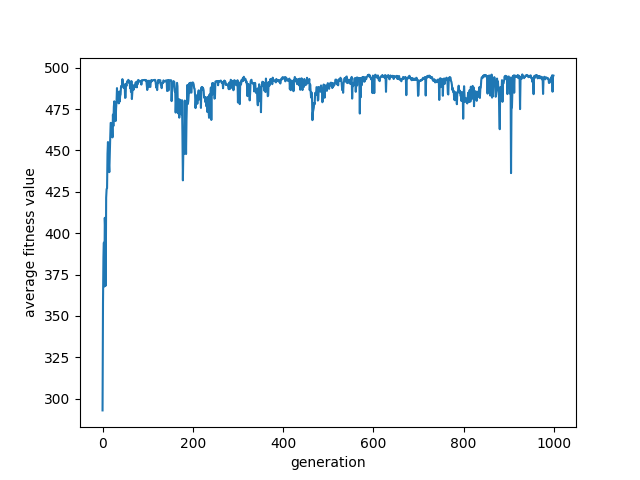
\includegraphics[width=0.7\textwidth]{../Images/average-fitness-value.png}
        \caption{The average fitness value among all the generations}
        \label{average-fitness-value}
    \end{figure}
    The best chromosome that I got is the following:
    \begin{align*}
        [ & 0, 0, 1, 1, 0, 1, 0, 1, 0, 0, 0, 0, 1, 1, 0, 0, 0, 0, 1, 0, \\
          & 1, 0, 0, 0, 0, 0, 1, 0, 0, 0, 0, 0, 1, 1, 1, 0, 0, 1, 1, 0, \\
          & 0, 0, 0, 0, 1, 1, 1, 0, 1, 1, 1, 1, 1, 0, 1, 0, 0, 1, 1, 0, \\
          & 1, 1, 1, 0, 0, 0, 0, 0, 0, 1 ]
    \end{align*}
    and the fitness value associated to it is 498 (this means that using this strategy you one can attain a score of \(600 - 498 = 102\) points, playing 100 games against a \emph{tit-for-tat} player).\par
    As you can see in figure \ref{average-fitness-value}, the average fitness value among all the generations increase quickly at the beginning and then remains more or less stable (the instability is due to the fact that sometimes random mutations occur). Moreover, the figure shows how the average fitness value is really closed to the best one: this means that the population is uniform and "similar" to the best chromosome.
\end{proof}